\documentclass[aspectratio=169,11pt]{beamer}
\usepackage{luatexja}
\usepackage{listings}
\usepackage{graphicx}
\usepackage{array,booktabs}
\lstset{basicstyle=\ttfamily\footnotesize,frame=single,breaklines=true,columns=fullflexible,keepspaces=true}
\usetheme{Madrid}
\usecolortheme{seahorse}
\setbeamertemplate{navigation symbols}{}
\newcommand{\sess}[3]{%
\begin{frame}{#1}
\textbf{このコマの目標}：#2

\vspace{0.6em}
\textbf{90分の進め方}
\begin{itemize}
#3
\end{itemize}
\end{frame}}
\title{Pythonによるデータ可視化}
\subtitle{――初めての人向け・90分$\times$8コマ――}
\author{講師用・受講者用 共通資料}
\date{想定日程：1日目 4コマ／2日目 4コマ}
\begin{document}

\begin{frame}
\titlepage
\begin{center}
\small 実習環境は Thonny（無料の初心者向けPython環境）を使います。\\
表もグラフも、pandas という道具箱で扱います。
\end{center}
\end{frame}

\begin{frame}{この講座でできるようになること}
\begin{itemize}
\item 平均などの「要約の数字」では見えない、データの姿をグラフで確かめられます
\item 目的に合ったデータの集め方と、変数の尺度に合った扱い方が分かります
\item pandas で表を作り、「伝わるグラフ」を描けます
\item データを眺めて気づいたことを、グラフだけで人に納得させられます
\item 「仮説を納得させるには、どんなデータが要るか」を考えられます
\end{itemize}
\vspace{0.5em}
合言葉は「\textbf{まず眺める。要約の前に、姿を見る}」です。\\
なお、統計的な検定はこの講座では扱いません。姿を見て、言葉で説明できるところまでが目標です。
\end{frame}

\begin{frame}{全8コマの地図}
\begin{center}
\begin{tabular}{clp{7.8cm}}
\toprule
コマ & テーマ & 内容 \\
\midrule
1 & データ可視化（導入編） & なぜグラフにするのか、姿を見るということ \\
2 & Python入門 & Thonnyと、最低限の文法 \\
3 & データ集めと尺度 & データの集め方、変数の尺度 \\
4 & 表のいろいろ & pandasによる表作成 \\
5 & グラフのいろいろ & pandasによるグラフ作成と伝わるデザイン \\
6 & データ分析 & 眺めて気づき、グラフだけで納得させる \\
7 & 仮説のためのデータ集め & 納得させるグラフに要るデータを考える \\
8 & テスト & データを眺め、気づきをグラフで納得させる \\
\bottomrule
\end{tabular}
\end{center}
\end{frame}

% ================= 第1コマ =================
\section{第1コマ}
\sess{第1コマ　データ可視化（導入編）}{「なぜグラフにするのか」を、実物を見て納得する}
{\item 講義（40分）：要約の数字の限界と、グラフの力
\item 演習（40分）：図を見て、姿を言葉にする
\item まとめ（10分）}

\begin{frame}{なぜ「グラフ」にするのか}
\begin{itemize}
\item 平均や合計のような「要約の数字」は便利ですが、それだけではデータの姿は分かりません
\item グラフにすると、増えた・減った・ばらつき・偏り・飛び抜けた値が一目で分かります
\item つまり可視化とは、\textbf{データが「どんなデータなのか」を納得できる形で知る}ための手段です
\item 姿が分かって初めて、他の人に伝えることができます。順番が大切です
\end{itemize}
\end{frame}

\begin{frame}{平均が同じでも、姿はこんなに違う}
\begin{center}
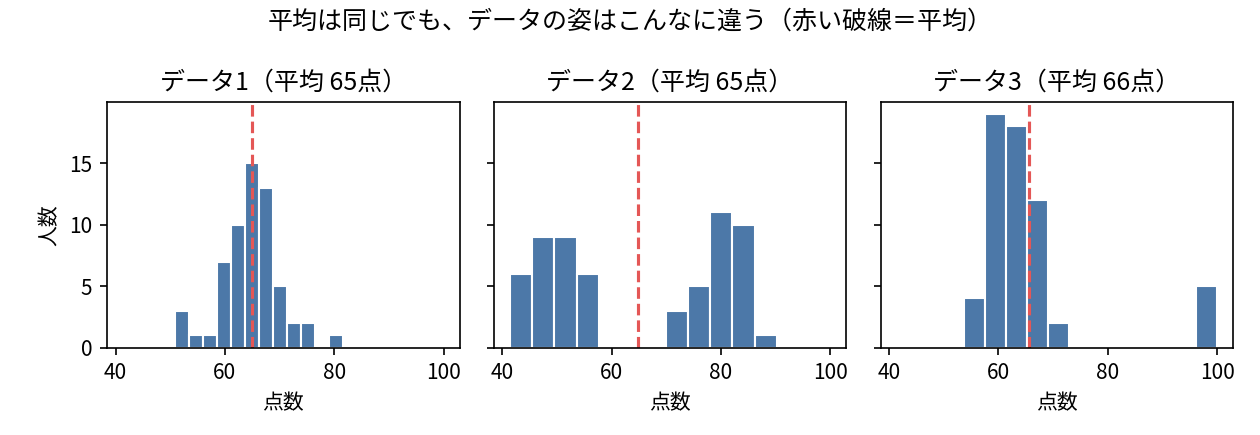
\includegraphics[width=0.86\textwidth]{assets/ex_same_mean.png}
\end{center}
\begin{itemize}
\item 3つのデータは平均がどれも約65点。でも、真ん中に集まる／得意・苦手に分かれる／飛び抜けた満点が混ざる、と姿は別物です
\item 「平均65点のクラス」という一言では、この違いは伝わりません
\end{itemize}
\end{frame}

\begin{frame}{姿が見えると、言葉が変わる}
\begin{center}
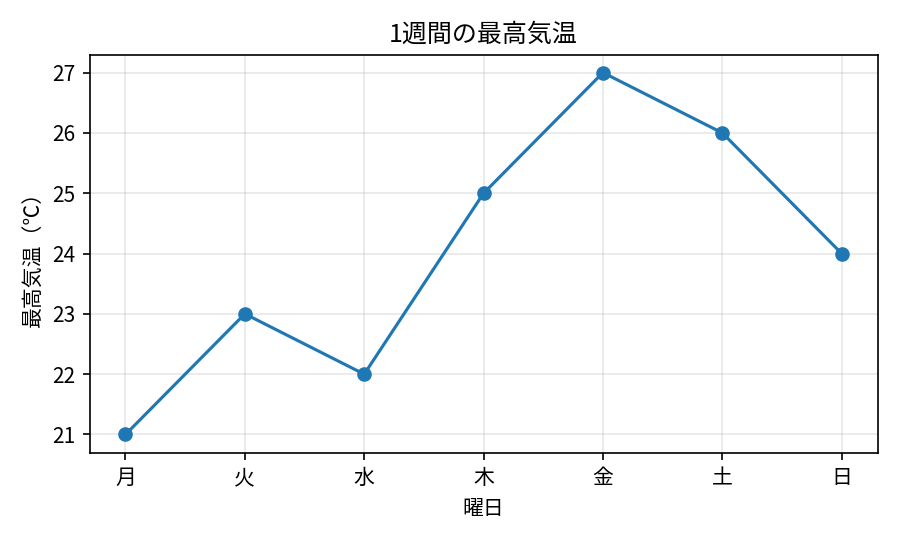
\includegraphics[width=0.56\textwidth]{assets/ex_line.png}
\end{center}
\begin{itemize}
\item 左の数字の並びを「金曜が一番暑かった」と言えるのは、姿を見たからです
\item この講座で繰り返すのは、この「眺めて、姿を言葉にする」作業です
\end{itemize}
\end{frame}


\begin{frame}{この講座の約束}
\begin{itemize}
\item エラーは失敗ではなく、先生からのヒントです
\item いきなり計算しない。まず眺める
\item グラフには「何を見せたいか」を必ず添える
\item 言えることと言えないことを分ける（相関と原因は別、など）
\end{itemize}
\vspace{0.5em}
\textbf{第1コマのまとめ}：可視化の動機は「データの何がどんななのかを、納得して知ること」です。
\end{frame}

% ================= 第2コマ =================
\section{第2コマ}
\sess{第2コマ　Python入門}{Thonnyでプログラムを書き、実行し、直せる}
{\item 実習（25分）：Thonnyの準備と実行
\item 講義と実習（40分）：変数、リスト、辞書、繰り返し、関数
\item 演習（20分）
\item まとめ（5分）}

\begin{frame}[fragile]{Thonny の準備}
\begin{itemize}
\item Thonny は、Python本体と編集画面が一緒になった、初心者向けの無料ソフトです
\item インストールは、Windowsのターミナル（PowerShell）で次の1行を実行します（講座前に済ませておきましょう）
\begin{lstlisting}
winget install AivarAnnamaa.Thonny
\end{lstlisting}
\item うまくいかない場合は、公式サイト \texttt{thonny.org} からも入手できます
\item コードは上の広い画面に書き、緑の $\blacktriangleright$ ボタン（または F5キー）で実行します。結果は下の画面に出ます
\item ファイルは名前をつけて保存します（例：\texttt{session2.py}）。配布ファイルは同じフォルダに置くのが約束です
\end{itemize}
\begin{lstlisting}
# 最初にこれを書いて、実行してみましょう
print("こんにちは、Python!")
print(1 + 2)
\end{lstlisting}
\end{frame}

\begin{frame}{Thonny の画面}
\begin{columns}
\begin{column}{0.58\textwidth}
\begin{center}
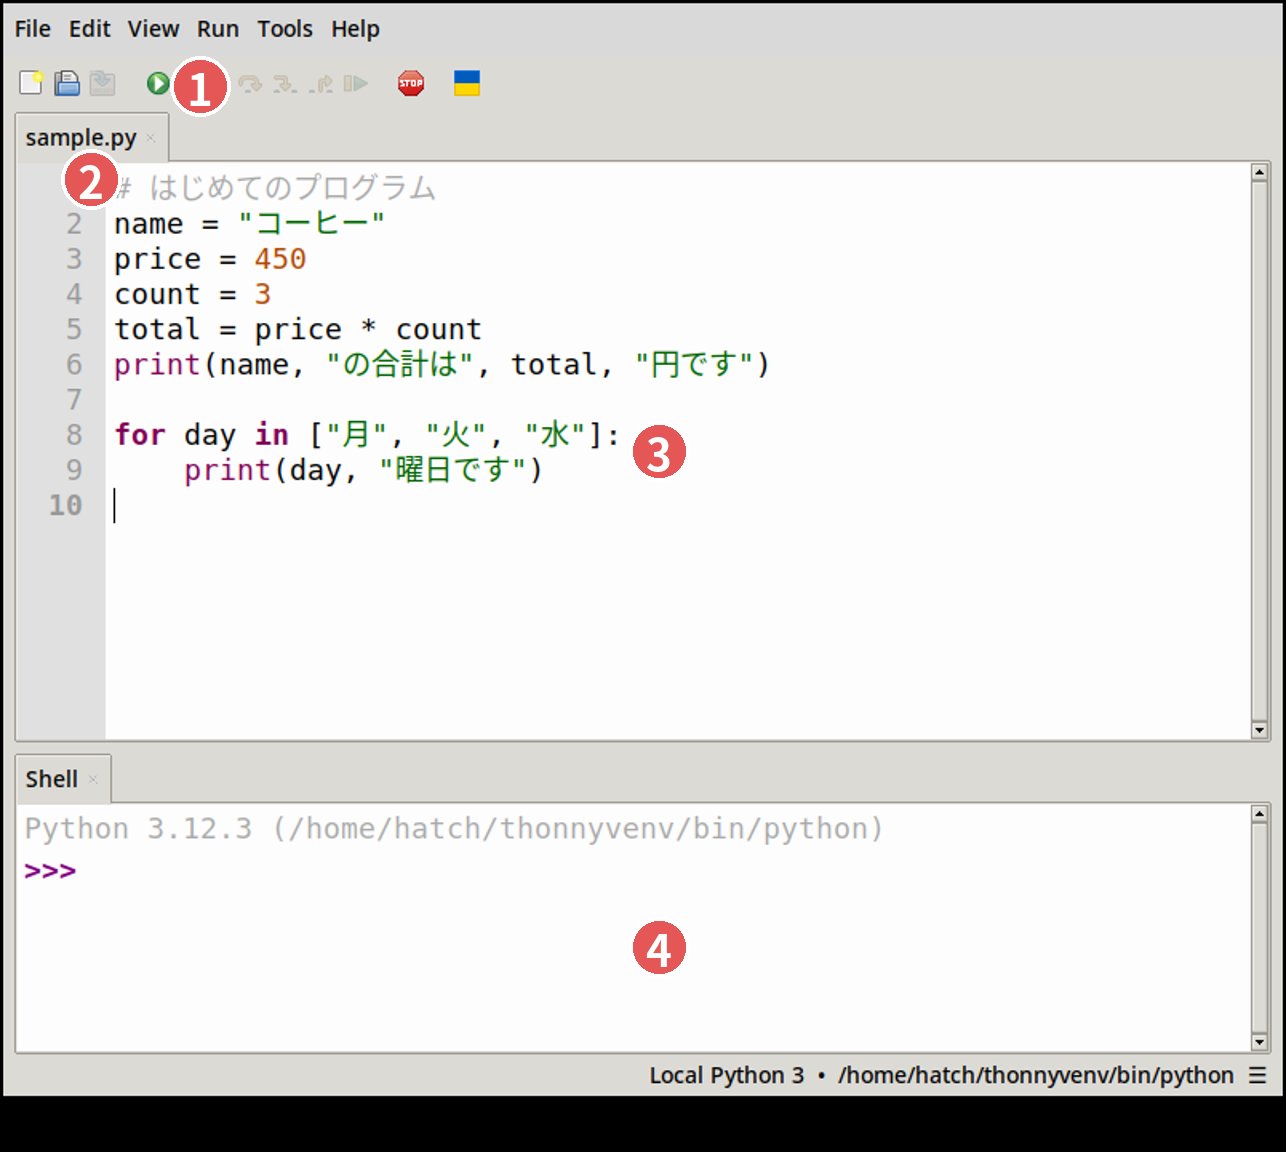
\includegraphics[width=\textwidth]{assets/thonny_ui.png}
\end{center}
\end{column}
\begin{column}{0.40\textwidth}
\begin{itemize}
\item[\textcolor{red}{1}] \textbf{実行ボタン}（緑の$\blacktriangleright$）：押すとプログラムが動きます。F5キーでも同じです
\item[\textcolor{red}{2}] \textbf{ファイルのタブ}：今開いているファイルの名前。複数開いて切り替えられます
\item[\textcolor{red}{3}] \textbf{編集エリア}：ここにプログラムを書きます。行番号が目印です
\item[\textcolor{red}{4}] \textbf{シェル}：実行結果やエラーメッセージが出る場所です
\end{itemize}
\vspace{0.4em}
（画面は一例です。表示はパソコンの設定で少し違うことがあります）
\end{column}
\end{columns}
\end{frame}

\begin{frame}{基本の使い方：4つのステップ}
\begin{enumerate}
\item \textbf{書く}：編集エリアにプログラムを書く
\item \textbf{保存する}：Ctrl+S。名前は「\texttt{session2.py}」のように、末尾が \texttt{.py} になるようにします
\item \textbf{実行する}：緑の$\blacktriangleright$ボタン、または F5キー
\item \textbf{結果を見る}：文字の結果はシェルに、グラフは新しいウィンドウに表示されます。エラー（赤い文字）が出たら、シェルの一番下の行がヒントです
\end{enumerate}
\vspace{0.5em}
追加の部品（pandas や japanize-matplotlib）は、メニューの「ツール → パッケージを管理」から入れることができます。第3コマ以降で使います。
\end{frame}

\begin{frame}[fragile]{変数：名前のついた箱}
\begin{lstlisting}
price = 450        # 数字を入れる
name = "コーヒー"   # 文字は " " で囲む
total = price * 3  # 箱の中身で計算できる
print(name, total) # コーヒー 1350
\end{lstlisting}
\begin{itemize}
\item \texttt{=} は「右のものを左の箱に入れる」という意味です（数学の＝とは少し違います）
\item \texttt{print} は「画面に出して」というお願いです
\item 「\texttt{\#}」の右側はメモ（コメント）。実行されません
\end{itemize}
\end{frame}

\begin{frame}[fragile]{リストと辞書}
\begin{lstlisting}
sales = [120, 85, 64, 42]   # 並んだデータ
print(sales[0])   # 120 ← 数え方は 0 から!
print(len(sales)) # 4
print(sum(sales)) # 合計

row = {"商品": "コーヒー", "単価": 450, "個数": 12}  # 辞書
print(row["商品"], row["単価"] * row["個数"])
\end{lstlisting}
辞書は「名前つきの箱の集まり」で、表の1行分のイメージです。第4コマの表につながります。
\end{frame}

\begin{frame}[fragile]{繰り返しと条件分岐}
\begin{lstlisting}
for day in ["月", "火", "水"]:
    print(day, "曜日です")

temp = 27
if temp >= 30:
    print("真夏日です")
elif temp >= 25:
    print("夏日です")
else:
    print("過ごしやすい日です")
\end{lstlisting}
\texttt{for} の下の行は、頭に空白（インデント）を4つ入れます。これが「繰り返す範囲」の印です。
\end{frame}

\begin{frame}[fragile]{関数：よく使う作業に名前をつける}
\begin{lstlisting}
def tax_included(price):
    return price * 1.1

print(tax_included(450))  # 495.0
\end{lstlisting}
\begin{itemize}
\item \texttt{def} で「新しいお願い」を作れます。\texttt{return} が答えの返し方です
\item エラー（赤い文字）が出たら、一番下の行に間違いの場所が書かれています。かっこの閉じ忘れ、スペル違い、全角文字の混入がよくある原因です
\end{itemize}
\end{frame}

\begin{frame}{第2コマの演習とまとめ}
\textbf{演習}
\begin{enumerate}
\item リスト \texttt{[80, 90, 70, 100]} の平均を、\texttt{sum} と \texttt{len} で求めましょう
\item 辞書で「自分の好きな商品」の1行を作り、単価×個数を表示しましょう
\item 繰り返しで、1から5までの2倍の数を順に表示しましょう
\end{enumerate}
\vspace{0.5em}
\textbf{まとめ}：変数＝箱、リスト＝並び、辞書＝名前つきの行、\texttt{for}＝繰り返し、\texttt{def}＝自作のお願い。この5つで足ります。
\end{frame}

% ================= 第3コマ =================
\section{第3コマ}
\sess{第3コマ　データ集め、データ（変数）の尺度}{データの集め方を選び、変数の尺度に合った扱いができる}
{\item 講義（35分）：データはどこから来るか
\item 講義（30分）：変数の尺度（4つのものさし）
\item 演習（20分）：身の回りの変数の尺度を当てる
\item まとめ（5分）}

\begin{frame}{データはどこから来るか}
\begin{itemize}
\item \textbf{調査}：アンケートやインタビューで人に聞く
\item \textbf{観察}：数える、測る、記録する（来客数、気温、所要時間）
\item \textbf{実験}：条件を変えて結果を比べる（肥料の有無で育ち方、など）
\item \textbf{既存の記録・公開データ}：売上記録、政府統計 e-Stat、自治体のオープンデータ
\item \textbf{機械の記録}：センサー、歩数計、アクセス記録
\end{itemize}
\vspace{0.5em}
どの集め方にも得手・不得手があります。「知りたいこと」に合った集め方を選ぶのが第一歩です。
\end{frame}

\begin{frame}{集めるときの注意（第7コマへの伏線）}
\begin{itemize}
\item \textbf{誰から集めたか}：一部の人だけに聞くと、答えが偏ります（例：常連だけに聞いた満足度）
\item \textbf{いくつ集めたか}：少なすぎると、偶然に振り回されます
\item \textbf{どう聞いたか}：質問の書き方で答えは変わります
\item 集めた条件（日時・場所・相手）を記録に残すことも、データの一部です
\end{itemize}
\end{frame}

\begin{frame}{標本という考え方}
\begin{itemize}
\item 本当に知りたい相手全体を\textbf{母集団}、実際に集めたデータの集まりを\textbf{標本（サンプル）}といいます
\item 例：本当は「この店の客全員」の満足度が知りたい。でも聞けるのは、今日来た30人だけ。この30人が標本です
\item 私たちが眺めるデータは、たいてい標本です。標本で見えた姿が、そのまま母集団の姿とは限りません
\item だからこそ「誰から・いくつ集めたか」が効いてきます。偏った標本からは、偏った姿しか見えません
\item この講座では、結論はまず「この標本ではこう見えた」と言える範囲に置きます。それでも、グラフで姿を示すことには大きな意味があります
\end{itemize}
\end{frame}

\begin{frame}{変数と尺度：データには「ものさし」がある}
\begin{itemize}
\item 変数とは、測ったり記録したりする項目のこと（身長、満足度、血液型、気温…）
\item 尺度とは、その変数がどんな性質の「ものさし」で測られているか、という区別です
\item 尺度が違うと、\textbf{やってよい計算や、合うグラフが変わります}
\end{itemize}
\begin{center}
\begin{tabular}{lp{5.4cm}p{5.6cm}}
\toprule
尺度 & 例 & イメージ \\
\midrule
名義尺度 & 血液型、商品名、天気 & 名札。区別だけ \\
順序尺度 & 順位、混雑具合、言葉の満足度（不満〜満足） & 順番はあるが間隔は不ぞろい \\
間隔尺度 & 気温（℃）、西暦、数値化した満足度 & 間隔は均等。0は「無」ではない \\
比尺度 & 身長、金額、個数 & 度量衡（長さ・重さなどの共通単位）。0＝本当に無い \\
\bottomrule
\end{tabular}
\end{center}
\end{frame}

\begin{frame}{尺度で「できること」が決まる}
\begin{center}
\begin{tabular}{lcccc}
\toprule
できること & 名義 & 順序 & 間隔 & 比 \\
\midrule
多い少ないの比較（順序） & × & ○ & ○ & ○ \\
平均を取る意味がある & × & $\triangle$ & ○ & ○ \\
差を言う（較べる：5℃差＝5℃差） & × & × & ○ & ○ \\
倍率を言う（比べる：2倍重い） & × & × & × & ○ \\
\bottomrule
\end{tabular}
\end{center}
\begin{itemize}
\item 血液型の「平均」は意味を持ちません。数えられるのは人数（度数）だけです
\item 満足度のように感覚を数値化したものは間隔尺度として扱い、平均も使います。ただし「4点は2点の2倍満足」とは言えません
\item 気温は差は言えても「今日は昨日の2倍暑い」とは言えません（0℃は「無」ではないから）
\end{itemize}
\end{frame}

\begin{frame}{比尺度は「度量衡」。数値データでも色々ある}
\begin{itemize}
\item まず言葉の説明です。\textbf{度量衡}（どりょうこう）は、昔からの「測るための共通のものさし」のことです。\textbf{度}＝長さ、\textbf{量}＝かさ（体積）、\textbf{衡}＝重さ。今で言えば、メートル・リットル・グラムといった単位の体系そのものを指します
\item \textbf{比尺度}の正体は、この度量衡です：長さ・重さ・時間・金額のように、誰がどこで測っても同じになる単位で測った数値です
\item 度量衡ではない数値データは、\textbf{間隔尺度}として扱います：満足度や「おいしさ 8点」のように、人の感覚を数値に割り振ったものです。差を言うことはできますが、「8点は4点の2倍おいしい」とは言えません
\item さらに注意したいのが\textbf{数字符号}：背番号、郵便番号、商品コードのように、質的データに数字を割り付けただけのもの。大小・強弱・優劣といった順序の意味がないので、数値でも\textbf{名義尺度として扱います}（「背番号の平均」は無意味です）
\end{itemize}
\end{frame}

\begin{frame}{水準と選択肢}
\begin{itemize}
\item \textbf{水準}とは、その変数が取りうる値（カテゴリ）のことです。例：天気の水準は「晴れ・くもり・雨」、血液型の水準は「A・B・O・AB」
\item アンケートで答えてもらう項目の並びを\textbf{選択肢}といいます。選択肢の作り方が、そのままデータの質を決めます
\item 選択肢の約束：漏れがない（「その他」を用意する）、重ならない、順序があるものは順序を保つ
\item 水準が文字列でも、順序があれば順序尺度です（例：「小さい・普通・大きい」「不満・やや不満・普通・やや満足・満足」）。これらは、1・2・3…と\textbf{数値に割り振り直して、間隔尺度として扱っても構いません}
\end{itemize}
\end{frame}

\begin{frame}{尺度とグラフの相性}
\begin{center}
\begin{tabular}{lp{8.8cm}}
\toprule
変数の組み合わせ & 合う表し方 \\
\midrule
名義尺度どうし & 人数を数える表（度数）、棒グラフ \\
順序尺度 & 度数の棒グラフ、中央値で要約 \\
間隔・比尺度 & ヒストグラム、箱ひげ図、平均で要約 \\
時間の流れ＋量 & 折れ線グラフ \\
量と量の関係 & 散布図 \\
\bottomrule
\end{tabular}
\end{center}
「どんな尺度か」を先に確かめる習慣が、変なグラフを防ぎます。
\end{frame}

\begin{frame}{尺度とグラフの相性（例）}
\begin{center}
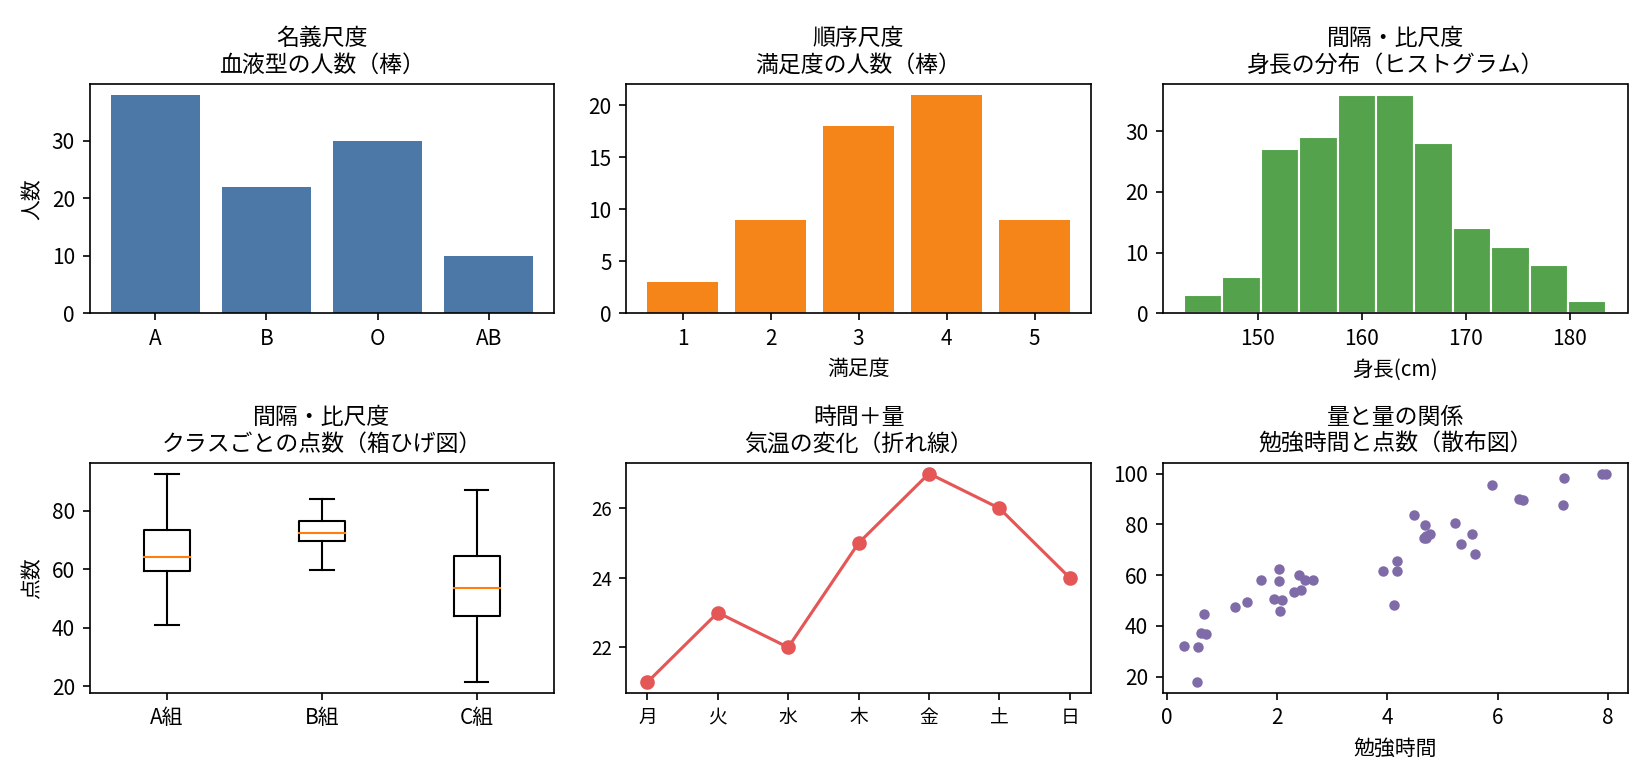
\includegraphics[width=0.76\textwidth]{assets/ex_scale_graphs.png}
\end{center}
\begin{itemize}
\item 名義・順序尺度は「人数を数えて棒グラフ」が基本。平均の棒グラフにはしません
\item 間隔・比尺度は分布を見るヒストグラムや箱ひげ図、時間の流れは折れ線、2つの量の関係は散布図です
\end{itemize}
\end{frame}

\begin{frame}{第3コマの演習とまとめ}
\textbf{演習：次の変数の尺度を当ててみましょう}
\begin{enumerate}
\item 郵便番号、好きな色、テストの点数、兄弟の人数、駅の混雑具合（空いている／普通／混んでいる）
\item 「平均を取ってよいか」も一緒に考えましょう
\end{enumerate}
\vspace{0.5em}
\textbf{まとめ}
\begin{itemize}
\item データの集め方には、調査・観察・実験・既存記録・機械の記録がある
\item 尺度は4つ（名義・順序・間隔・比）。尺度が、できる計算と合うグラフを決める
\end{itemize}
\end{frame}

% ================= 第4コマ =================
\section{第4コマ}
\sess{第4コマ　表のいろいろ。pandasによる表作成}{目的に合った形の表を、pandasで作れる}
{\item 講義（25分）：表の4段階（収集・要約・関係・推測）
\item 一緒に実習（40分）：pandasの基本と集計
\item 演習（20分）：クロス集計を作る
\item まとめ（5分）}

\begin{frame}{表は「段階」ごとに姿が違う}
\begin{center}
\begin{tabular}{clp{7.6cm}}
\toprule
段階 & すること & 表の形 \\
\midrule
1 収集 & データを集める & \textbf{一覧表}：集めた記録そのもの \\
2 要約 & 集めたデータの様子を知る & \textbf{要約の表}：変数ごとに代表値・統計値に置き換える \\
3 関係 & データとデータの関係性を調べる & \textbf{クロス集計表（分割表）}：2つの変数の組み合わせ \\
4 推測 & ある値から別の値を推測する & \textbf{混同行列}：推測の正誤の数を数える表 \\
\bottomrule
\end{tabular}
\end{center}
同じ「表」でも、段階が進むにつれて姿が変わります。このコマでは、段階1〜3の表を pandas で作り、段階4の混同行列を紹介します。
\end{frame}

\begin{frame}{段階2：要約の表}
\begin{itemize}
\item 要約の表とは、変数ごとに値を「代表値や統計値」に置き換えた表です
\item 載せるのは、個数（データの数）、平均、中央値、第1・第3四分位数、最小・最大など
\item 一覧表のまま眺めるより、「だいたいどのあたりか」「どれくらい広がっているか」が掴めます
\item pandas では \texttt{describe()} が要約の表を一気に出してくれます（第5コマの四分位数とつながります）
\end{itemize}
\end{frame}

\begin{frame}[fragile]{pandas は「表とグラフの道具箱」}
\begin{itemize}
\item 表（DataFrame）をプログラムで扱うための道具箱です。Excelのシートを、そのまま計算できるようにしたもの、と考えてください
\item この講座では、表もグラフも pandas で通します
\item インストールは Thonny の機能で行います：メニュー「ツール → パッケージを管理」を開き、\texttt{pandas} を探して「インストール」を押します（初回のみ）。japanize-matplotlib も同じ場所から入れます
\item CSVファイル（カンマ区切りの表ファイル）を読み込むのが第一歩です
\end{itemize}
\begin{lstlisting}
import pandas as pd

df = pd.read_csv("data/weather_week.csv")
print(df.head())    # 最初の5行
print(df.shape)     # (行数, 列数)
print(df.columns)   # 列の名前
\end{lstlisting}
\end{frame}

\begin{frame}[fragile]{列を取り出す・条件で絞る・列を足す}
\begin{lstlisting}
print(df["最高気温"].max())    # 最大値
print(df["最高気温"].mean())   # 平均

hot = df[df["最高気温"] >= 25]  # 条件に合う行だけ
print(hot)

sales["金額"] = sales["単価"] * sales["個数"]  # 新しい列
\end{lstlisting}
「まず眺める」が鉄則です。いきなり集計せず、\texttt{head} で中身を確認します。
\end{frame}

\begin{frame}[fragile]{集計して一元表を作る}
\begin{lstlisting}
by_item = (sales.groupby("商品")["金額"].sum()
           .sort_values(ascending=False))
print(by_item)
\end{lstlisting}
\texttt{groupby} は「種類ごとに分けて、まとめる」作業です。Excelのピボットテーブルにあたります。
\end{frame}

\begin{frame}[fragile]{段階3：クロス集計表（分割表）を作る}
\begin{lstlisting}
survey = pd.read_csv("data/survey.csv")
cross = pd.crosstab(survey["年代"], survey["満足度"])
print(cross)
\end{lstlisting}
\begin{itemize}
\item 行（年代）と列（満足度）の交差するマスに人数が入ります。「年代によって満足度は違うか」のような、\textbf{関係}を調べる問いに答える形です
\item この形の表は「分割表」とも呼ばれます
\item 0 のマスは、その組み合わせのデータが無い、という意味です
\end{itemize}
\end{frame}

\begin{frame}[fragile]{段階4：推測と混同行列}
\begin{itemize}
\item 推測とは、あるデータの値から別のデータの値を当てることです。当てた結果の正しさを数えるのが、この段階の仕事です
\item 推測の出来を評価する表が\textbf{混同行列}です。クロス集計表に似ていますが、\textbf{行と列が同じカテゴリ}（実際 × 判断）なのが特徴で、斜めのマスが正解です
\item 心理学の\textbf{信号検出理論}が、その代表例です（次のページ）
\end{itemize}
\end{frame}

\begin{frame}{信号検出理論：刺激のあるなし × 反応のあるなし}
\begin{itemize}
\item かすかな音が「聞こえたか」を答える実験のように、刺激があるかないかと、反応（「あった」と答えたか）の組み合わせで、判断の様子を調べる理論です
\end{itemize}
\begin{center}
\begin{tabular}{lcc}
\toprule
実際 ＼ 反応 & 「あった」 & 「なかった」 \\
\midrule
刺激あり（50試行） & 38 \textbf{ヒット} & 12 \textbf{見落とし} \\
刺激なし（50試行） & 9 \textbf{誤警報} & 41 \textbf{正棄却} \\
\bottomrule
\end{tabular}
\end{center}
\begin{itemize}
\item この人の的中の様子：刺激ありでは76\%当て、刺激なしでは18\%「あった」と言ってしまう
\item 判断の基準がゆるい人は「ヒットも誤警報も多い」、厳しい人は「見落としが多い」といった具合に、4つのマスのバランスに、その人の判断のクセが表れます
\item この表はまさに混同行列です。pandas では \texttt{pd.crosstab(刺激の列, 反応の列)} で作れます
\end{itemize}
\end{frame}

\begin{frame}{第4コマの演習とまとめ}
\textbf{演習}
\begin{enumerate}
\item \texttt{weather\_week.csv} の最低気温の平均と、降水量が0より大きい日の一覧を作りましょう
\item \texttt{shop\_sales.csv} で、商品ごとの「個数」の合計の一元表を作りましょう
\item \texttt{survey.csv} で年代×満足度のクロス集計を作り、気づいたことを1つ書きましょう
\end{enumerate}
\vspace{0.5em}
\textbf{まとめ}：表は段階で姿が変わる（収集＝一覧表、要約＝代表値の表、関係＝クロス集計表（分割表）、推測＝混同行列）。pandas の主役は \texttt{describe}、\texttt{groupby}、\texttt{crosstab} です。
\end{frame}

% ================= 第5コマ =================
\section{第5コマ}
\sess{第5コマ　グラフのいろいろ。伝わるデザイン}{尺度と目的に合ったグラフを選び、誤解なく伝わる形に仕上げられる}
{\item 講義（25分）：グラフの種類と選び方
\item 一緒に実習（35分）：pandasのグラフ機能
\item 講義と実習（25分）：伝わるデザイン
\item まとめ（5分）}

\begin{frame}{グラフは「知りたいこと」で選ぶ}
\begin{center}
\begin{tabular}{lp{8.6cm}}
\toprule
知りたいこと & 合うグラフ \\
\midrule
時間とともにどう変わったか & 折れ線グラフ \\
量を比べたい（名義・順序） & 棒グラフ \\
2つの量に関係があるか & 散布図 \\
ばらつき・偏りを見たい & ヒストグラム \\
複数のグループの分布を比べたい & 箱ひげ図 \\
全体の中の割合 & 円グラフ／100\%積み上げ棒（注意あり） \\
\bottomrule
\end{tabular}
\end{center}
第3コマの尺度とセットで考えます。「格好いいから」ではなく「質問に答える形」を選ぶのが原則です。
\end{frame}

\begin{frame}{各グラフは「何の、どんな様子」を見せるか}
\begin{center}
\begin{tabular}{lp{9.6cm}}
\toprule
グラフ & 何の、どんな様子を見せたいときに使うか \\
\midrule
棒グラフ & カテゴリごとの\textbf{量の大きさ}。「どのカテゴリが、どれくらい大きいか」の様子 \\
ヒストグラム & 1つの量の\textbf{分布の形}。「どこに集まり、どう偏り、山はいくつか、飛び抜けた値はないか」の様子 \\
箱ひげ図 & 複数のグループの\textbf{分布の要約}。「中心はどこか、広がりはどうか、外れ値はあるか」をグループごとに比べる様子 \\
折れ線グラフ & 時間とともに量が\textbf{どう変化したか}。「増えた・減った・横ばいか、ピークはいつか」の様子 \\
散布図 & 2つの量の\textbf{関係}。「一方が大きいとき、もう一方も大きいか（右上がり／右下がり／無関係）、点はどう集まり、外れ値はないか」の様子 \\
\bottomrule
\end{tabular}
\end{center}
\vspace{0.3em}
描く前に「何の、どんな様子を見せたいのか」を一言で言えることが、グラフ選びの出発点です。
\end{frame}

\begin{frame}[fragile]{pandas のグラフは「表から直接」}
\begin{lstlisting}
import pandas as pd
import matplotlib.pyplot as plt
import japanize_matplotlib  # 日本語表示(初回のみ。Thonnyの「ツール→パッケージを管理」から入れる)

temp.plot.line(marker="o", title="1週間の最高気温", ylabel="最高気温(℃)")
sales.plot.bar(title="飲み物の売上", ylabel="杯数")
study.plot.scatter(x="勉強時間", y="点数")
plt.show()  # 表示する(仕上げは matplotlib が担当)
\end{lstlisting}
\begin{itemize}
\item 集計した表（SeriesやDataFrame）に \texttt{.plot} をつけるだけです
\item pandas のグラフは裏側で matplotlib が描いています。表示や細かい仕上げは matplotlib の仕事、と覚えてください
\item 保存は \texttt{plt.savefig("名前.png")} を \texttt{show()} の前に書きます
\end{itemize}
\end{frame}

\begin{frame}[fragile]{折れ線・棒・散布図}
\begin{lstlisting}
temp.plot.line(marker="o")       # 折れ線:変化を見る
sales.plot.bar(color="#4C78A8")  # 棒:比べる
study.plot.scatter(x="勉強時間", y="点数")  # 散布:関係を見る
heights.plot.hist(bins=12)       # ヒスト:分布を見る
\end{lstlisting}
\begin{center}
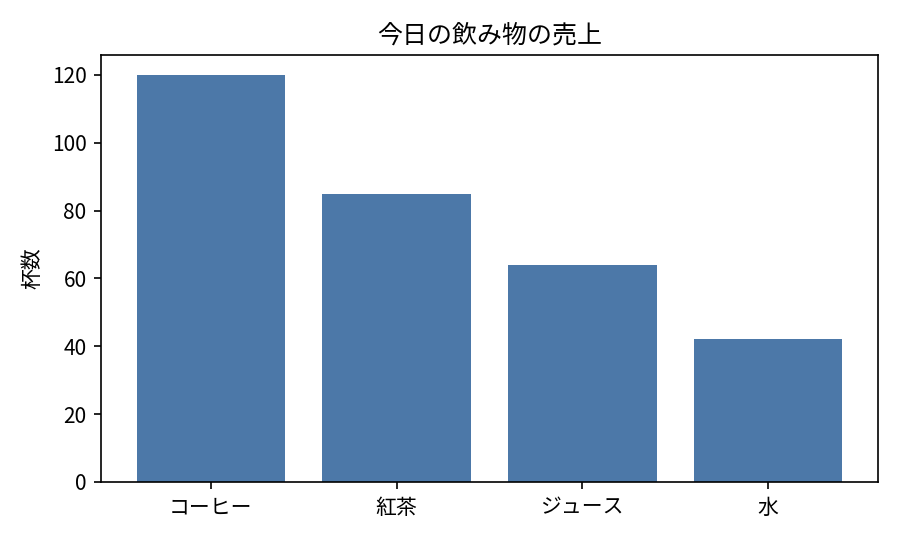
\includegraphics[width=0.44\textwidth]{assets/ex_bar.png}
\end{center}
\end{frame}

\begin{frame}[fragile]{箱ひげ図：分布を要約して比べる}
\begin{lstlisting}
scores.boxplot()   # 列ごとに箱ひげ図が並ぶ
plt.title("クラスごとのテストの点数")
plt.ylabel("点数")
plt.show()
\end{lstlisting}
\begin{center}
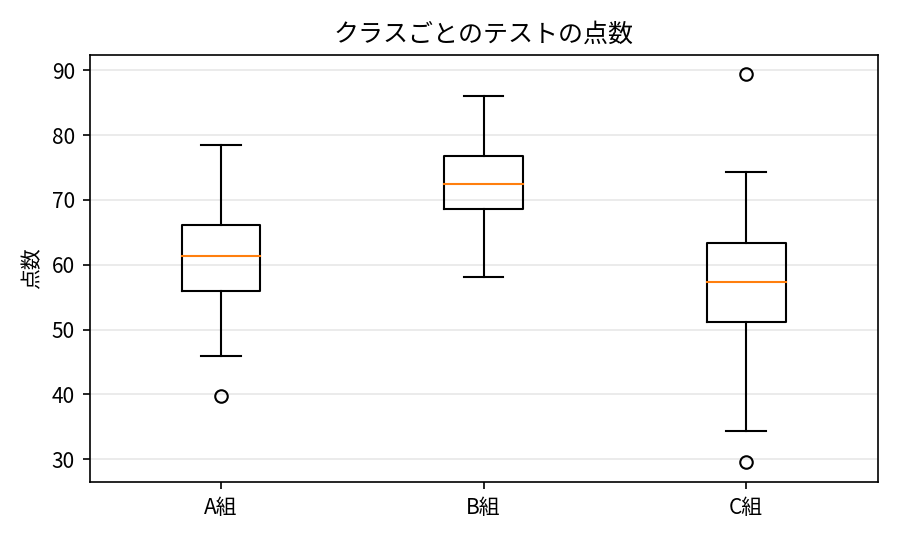
\includegraphics[width=0.40\textwidth]{assets/ex_box.png}
\end{center}
\end{frame}

\begin{frame}{四分位数：データを小さい順に「4つに分ける」}
\begin{itemize}
\item データを小さい順に並べたとき、下から25\%の位置の値が\textbf{第1四分位数（Q1）}、50\%が\textbf{中央値}、75\%が\textbf{第3四分位数（Q3）}です
\item 箱の長さにあたる Q3$-$Q1 を\textbf{四分位範囲（IQR）}といい、「真ん中50\%の広がり」を表します
\item 例（あるクラス25人の点数）：Q1＝60点、中央値＝66点、Q3＝73点、IQR＝13点
\item 平均と違い、四分位数は飛び抜けた値に引きずられにくいのが特長です
\item なお、境界の細かい計算には流儀がいくつかあり、手計算とソフトの値が少しずれることがあります。考え方（並べて4つに分ける）が大事です
\end{itemize}
\end{frame}

\begin{frame}{箱ひげ図の描き方}
\begin{columns}
\begin{column}{0.52\textwidth}
\begin{center}
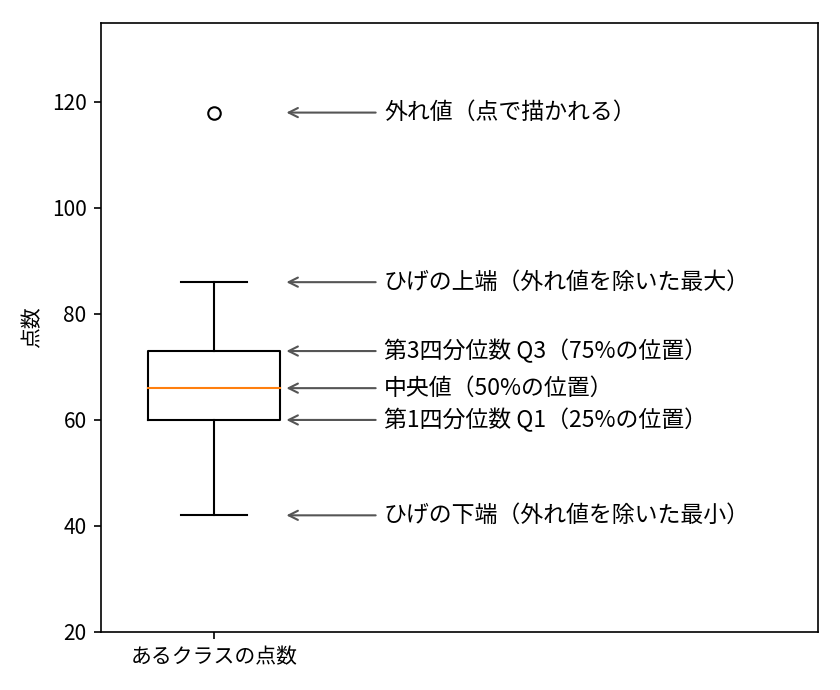
\includegraphics[width=\textwidth]{assets/ex_box_anatomy.png}
\end{center}
\end{column}
\begin{column}{0.46\textwidth}
\textbf{描く手順}
\begin{enumerate}
\item データを小さい順に並べ、Q1・中央値・Q3 を求める
\item Q1からQ3までを「箱」として描き、中央値に線を引く
\item ひげは、外れ値を除いた最小・最大まで伸ばす
\item 外れ値は、点で別に描く
\end{enumerate}
\vspace{0.4em}
箱が短い＝真ん中半分が集まっている、箱が長い＝ばらついている、と読みます。
\end{column}
\end{columns}
\end{frame}

\begin{frame}{外れ値（ハズレ値）：飛び抜けた値の扱い}
\begin{itemize}
\item 箱ひげ図では、目安として「Q1 $-$ 1.5$\times$IQR より小さい値」「Q3 $+$ 1.5$\times$IQR より大きい値」を外れ値として点で描きます
\item 例：Q1＝60、Q3＝73、IQR＝13 のとき、境界は 40.5点と 92.5点。118点は外れ値になります
\item 外れ値は「間違い」と決めつけないでください。記録ミスのこともあれば、本物の珍しい出来事（イベント日、特別な客）のこともあります
\item 見つけたら、まず「なぜこの値なのか」を調べる。消すのは、その理由が分かってからです
\end{itemize}
\end{frame}

\begin{frame}{箱ひげ図の読み方・円グラフの注意}
\begin{itemize}
\item 箱の真ん中の線が\textbf{中央値}、箱の上下端が下から25\%・75\%の位置、ひげが全体の広がり、ひげの外の点が飛び抜けた値の候補です
\item ヒストグラムが「1つの分布の形」、箱ひげ図は「分布の要約を並べて比べる」道具です
\item 円グラフは項目が3〜4個まで、割合の差が大きいときだけ。似た割合の比較は棒グラフが正確です
\item 3Dグラフは奥行きで値が読みにくくなるため、この講座では扱いません
\end{itemize}
\end{frame}

\begin{frame}{惑わせるグラフの典型}
\begin{center}
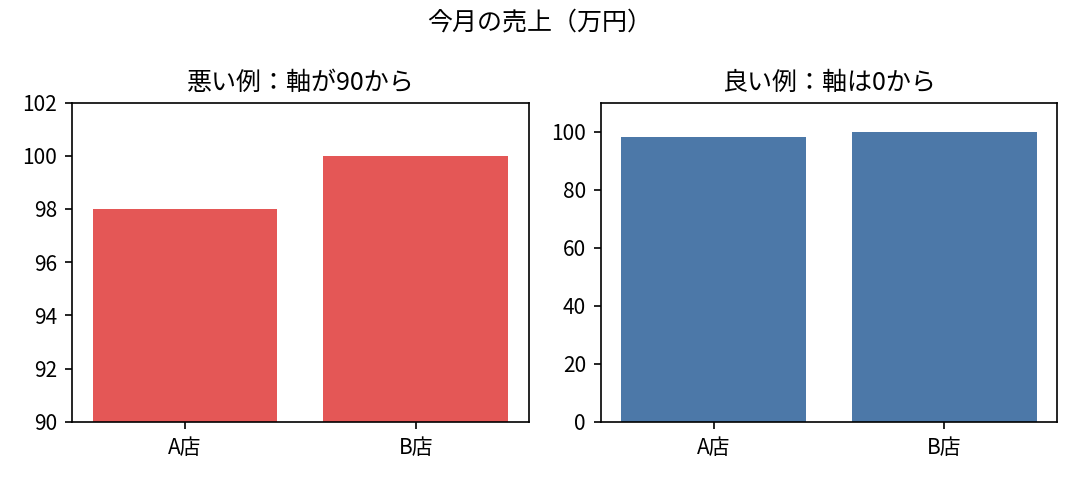
\includegraphics[width=0.66\textwidth]{assets/ex_axis.png}
\end{center}
\begin{itemize}
\item 98万円と100万円の差が、左では「何倍も違う」ように見えます。原因は縦軸が0から始まっていないこと
\item 棒グラフの軸は\textbf{0から}が決まりです。ほかにも「都合のよい期間だけ切り取る」「目盛りの幅をそろえない」などが典型です
\end{itemize}
\end{frame}

\begin{frame}[fragile]{伝わるデザインの決まり}
\begin{itemize}
\item 色は「飾り」ではなく「区別」のため。強調したいものだけ濃い色、あとは灰色が効果的です
\item 一番伝えたい点には、言葉と矢印の注釈を（\texttt{ax.annotate}）
\item タイトルは「1週間の最高気温」より「週の後半に暑くなった」のように、\textbf{結論（主張）を書く}と伝わります
\end{itemize}
\begin{lstlisting}
sales.plot.bar(color=["gray", "gray", "#E45756", "gray"],
               title="ジュースの売上が伸びている")
ax = temp.plot.line(marker="o", title="週の後半に暑くなった")
ax.annotate("今週の最高", xy=("金", 27), xytext=("水", 28),
            arrowprops=dict(arrowstyle="->"))
\end{lstlisting}
\end{frame}

\begin{frame}[fragile]{複数のグラフを並べる}
\begin{lstlisting}
fig, axes = plt.subplots(2, 2, figsize=(8, 6))
temp.plot.line(ax=axes[0, 0], marker="o")
sales.plot.bar(ax=axes[0, 1])
study.plot.scatter(ax=axes[1, 0], x="勉強時間", y="点数")
heights.plot.hist(ax=axes[1, 1], bins=12)
plt.tight_layout()
plt.show()
\end{lstlisting}
比べたいもの、補い合うものを並べると、1枚で話が完結します（例図は次のページ）。
\end{frame}

\begin{frame}{第5コマの演習とまとめ}
\textbf{演習}
\begin{enumerate}
\item お題（出席率の変化／満足度の偏り／身長と体重の関係）に合うグラフを選んで描きましょう
\item 縦軸が90から始まる棒グラフを作り、0からに直して印象の違いを確認しましょう
\item 自分のグラフのタイトルを「結論を書く形」に書き換えましょう
\end{enumerate}
\vspace{0.5em}
\textbf{まとめ}：選び方は「尺度×知りたいこと」。デザインの目的は格好よさではなく、誤解なく伝わることです。
\end{frame}

% ================= 第6コマ =================
\section{第6コマ}
\sess{第6コマ　データを眺めて、気づいたことをグラフだけで納得させる（データ分析）}{配布データを眺めて気づきを見つけ、それをグラフだけで人に伝える}
{\item 講義（15分）：分析の進め方
\item 一緒に実習（35分）：反応時間のデータで気づきを探す
\item 演習（35分）：グラフだけで納得させる1枚を作る
\item まとめ（5分）}

\begin{frame}{分析の進め方}
\begin{enumerate}
\item \textbf{眺める}：一覧表、基本の集計、いろいろなグラフで姿を見る
\item \textbf{気づきをメモする}：「音楽があると遅そう」「年代で違いそう」のように、仮の言葉でよい
\item \textbf{確かめる}：気づきに合った表（集計）とグラフを作り直す。比べるときは平均だけでなく\textbf{分布}を見る（次のページ）
\item \textbf{納得させる}：説明文ではなく、グラフそのもの（タイトル＝主張、注釈、並べ方）で伝える
\end{enumerate}
\vspace{0.5em}
この順番が逆（いきなり結論）にならないことが大切です。また、手元のデータは「標本（サンプル）」です。全体の話に広げるときは、その意識を持ちましょう（第3コマ）。
\end{frame}

\begin{frame}{比べるときは「分布の格差」で見る}
\begin{center}
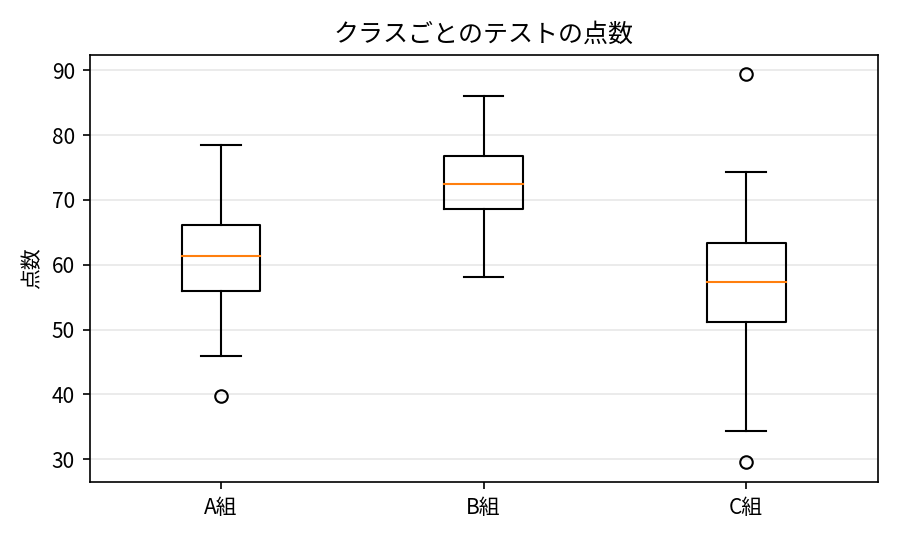
\includegraphics[width=0.40\textwidth]{assets/ex_box.png}
\end{center}
\begin{itemize}
\item 平均が違っても、分布が大きく重なっていれば、姿の差は小さいかもしれません。逆に、平均が近くても分布の形が違えば、大きな違いかもしれません
\item 比べる観点は3つ：\textbf{中心の位置}（中央値）、\textbf{広がり}（ばらつき）、\textbf{重なり具合}
\item だから比較には、箱ひげ図やヒストグラムを\textbf{並べた図}が向いています。「平均○○ vs 平均△△」の数字の対決で終わらせないのが、この講座の流儀です
\end{itemize}
\end{frame}

\begin{frame}{実習データ：反応時間の実験（80名）}
\begin{itemize}
\item 列：ID、年代、条件（静か／音楽あり）、反応時間（ミリ秒）、正答数（20問中）（\texttt{psych\_rt.csv}）
\item 画面に合図が出たらボタンを押す、という課題を80名に実施した記録です
\item まず一覧を眺め、条件ごと・年代ごとの要約の表を作ってみましょう
\item どんな「気づき」が出てくるでしょうか
\end{itemize}
\vspace{0.5em}
講師デモで見つかる気づきの例は伏せておきます。自分の目で探すのがこのコマの主役です。
\end{frame}

\begin{frame}{「グラフだけで納得させる」ための工夫}
\begin{itemize}
\item タイトルに主張を書く：「曜日ごとの来客数」→「土日は平日の約1.5倍の来客」
\item 比べたいものを隣に並べる（平日と休日、晴れと雨）
\item 主張と関係ない要素はそぎ落とす（色は最小限、凡例は短く）
\item 数字を添える場所は1か所に絞る（注釈で代表値だけ）
\item 読み手が「本当かな？」と思う順番に、根拠のグラフを並べる
\end{itemize}
\end{frame}

\begin{frame}{第6コマの演習とまとめ}
\textbf{演習}
\begin{enumerate}
\item 反応時間のデータから、自分の「気づき」を1つ選ぶ
\item その気づきを、タイトル＝主張のグラフ1枚で表す（説明文は書かない）。比べる場合は、分布を並べた図にすること
\item 隣の人と見せ合い、「主張が一目で伝わるか」を確かめ合う
\end{enumerate}
\vspace{0.5em}
\textbf{まとめ}：分析とは「眺める → 気づく → 確かめる → グラフで納得させる」の往復です。
\end{frame}

% ================= 第7コマ =================
\section{第7コマ}
\sess{第7コマ　仮説を納得させるグラフを作るためのデータ集め}{仮説から逆算して、必要なデータの集め方を設計できる}
{\item 講義（30分）：仮説と「比べる相手」
\item 講義（25分）：偏りを避ける集め方
\item 実習（30分）：データ集め計画シートを作る
\item まとめ（5分）}

\begin{frame}{仮説とは}
\begin{itemize}
\item 仮説とは「もし○○なら、△△になるはず」という、確かめられる形の予想です
\item 例：「音楽があると反応が遅くなるはず」「練習を重ねると反応が速くなるはず」
\item あいまいな予想（「なんとなく速そう」）は、データで確かめられません
\item 納得させるグラフを作るには、\textbf{仮説に合ったデータ}が要ります。第6コマのように手元のデータを眺める段階とは、ここが違います
\end{itemize}
\end{frame}

\begin{frame}{納得には「比べる相手」が要る}
\begin{itemize}
\item 「音楽ありの反応時間は390ミリ秒でした」だけでは、遅いのか分かりません
\item 静かな条件（中央値339ミリ秒）と並べて初めて、「音楽があると遅い」と納得できます
\item 比べ方は仮説で決まります：静か vs 音楽あり／実施前 vs 実施後／若い年代 vs 高い年代
\item 計画の時点で「何と何を比べるか」を決めておくことが、集め方の設計です
\end{itemize}
\end{frame}

\begin{frame}{偏りを避ける}
\begin{itemize}
\item \textbf{相手の偏り}：常連だけ、若い人だけに聞くと、全体の姿になりません
\item \textbf{タイミングの偏り}：休日だけ、イベントの日だけを集めると偏ります
\item \textbf{聞き方の偏り}：「おいしかったですよね？」のような誘導は答えを歪めます
\item \textbf{数の不足}：数件だけでは偶然と区別がつきません。日々の記録なら、まず2週間〜1か月が目安です
\item 集めた条件（いつ・どこで・誰から・いくつ）を必ず記録に残します
\end{itemize}
\end{frame}

\begin{frame}{データ集め計画シート}
\begin{center}
\begin{tabular}{lp{9.4cm}}
\toprule
項目 & 書くこと \\
\midrule
仮説 & 「もし○○なら、△△になるはず」の一文 \\
比べる相手 & 何と何を比べれば納得できるか \\
必要な変数 & 測る項目と、その尺度（第3コマ） \\
集め方 & 調査／観察／実験／既存記録のどれか、具体的な手順 \\
相手と数 & 誰から・いくつ集めるか。偏りへの対策 \\
期間 & いつからいつまでか \\
\bottomrule
\end{tabular}
\end{center}
\end{frame}

\begin{frame}{第7コマの実習とまとめ}
\textbf{実習}
\begin{enumerate}
\item 班ごとに仮説を1つ立て、計画シートを完成させましょう
\item 既にあるデータ（反応時間の実験データなど）で「下見」ができる場合は、比べる表だけ作ってみましょう
\item 発表は「仮説」と「比べる相手」の2点を中心に
\end{enumerate}
\vspace{0.5em}
\textbf{まとめ}：良いグラフは、良いデータ集めから。仮説 → 比べる相手 → 集め方の順に設計します。
\end{frame}

% ================= 第8コマ =================
\section{第8コマ}
\sess{第8コマ　テスト}{配布データを眺めて気づきを見つけ、グラフで納得させる（評価）}
{\item 説明（10分）：課題と進め方
\item テスト（70分）：各自で取り組む
\item 自己チェック（10分）：提出前の確認}

\begin{frame}{テストの課題}
\textbf{課題文}：配布されたデータ（\texttt{test\_psych.csv}：ある注意課題の実験に参加した120名の記録）を眺めて、気づきを\textbf{1つ}挙げ、それを\textbf{グラフだけで納得させる}形で示しなさい。
\begin{itemize}
\item 列：ID、年代、性別、条件（単独／ペア）、時間帯（午前／午後）、反応時間（ミリ秒）、正答数（20問中）
\item 提出物：① 気づき（1文）② その気づきを納得させるグラフ（タイトル＝主張）③ 使ったプログラム
\item グラフの説明文は最小限に。タイトル、軸、注釈で伝えること
\item 比べる場合は、平均の数字だけでなく\textbf{分布の格差}（中心・広がり・重なり）が見える形にすること
\item 検定などの統計手法は不要です。この標本の姿として言える範囲で述べること
\end{itemize}
\end{frame}

\begin{frame}{評価の観点}
\begin{itemize}
\item 気づきが、データの姿に合っているか（飛躍がないか）
\item 気づきに合った表（集計）とグラフの形を選べているか。比較は分布で示せているか
\item タイトル＝主張、軸と単位、比べる相手の並べ方など、「納得させる工夫」があるか
\item プログラムが手元で再実行できるか
\end{itemize}
\vspace{0.5em}
分からなくなったら、第6コマの進め方（眺める → 気づく → 確かめる → 納得させる）に戻ってください。
\end{frame}

\begin{frame}{提出前チェックリスト}
\begin{itemize}
\item[$\square$] 気づきは1つに絞ってある
\item[$\square$] グラフのタイトルが主張になっている
\item[$\square$] 比べる場合は、分布の違い（中心・広がり・重なり）が見える
\item[$\square$] 軸ラベルと単位がそろっている
\item[$\square$] 棒グラフの軸が0から始まっている
\item[$\square$] 比べる相手が同じ図の中にいる
\item[$\square$] 画像として保存できる（\texttt{savefig} は \texttt{show} の前）
\end{itemize}
\end{frame}

% ================= 付録 =================
\section{付録}
\begin{frame}{付録A　困ったときの対処表}
\begin{center}
\begin{tabular}{lp{8.4cm}}
\toprule
症状 & 対処 \\
\midrule
真っ赤なエラーが出た & 一番下の行を読む。かっこ・スペル・全角文字を確認 \\
グラフが表示されない & \texttt{plt.show()} の書き忘れ。保存してから、もう一度実行（F5） \\
日本語が四角になる & japanize-matplotlib を使う（第5コマ） \\
変数が無いと言われる & プログラムは上から順に実行される。必要な行の位置を確認 \\
CSVが文字化け・見つからない & \texttt{encoding} の指定／プログラムと同じフォルダにあるか確認 \\
保存した図が見当たらない & \texttt{savefig} は \texttt{show} の前。同じフォルダを探す \\
\bottomrule
\end{tabular}
\end{center}
\end{frame}

\begin{frame}{付録B　用語のミニ辞典}
\begin{itemize}
\item \textbf{Thonny}：Python本体と編集画面が一緒になった初心者向けソフト。F5キーで実行する
\item \textbf{変数（統計）}：測ったり記録したりする項目。尺度（名義・順序・間隔・比）がある
\item \textbf{DataFrame}：pandasの表全体。Excelのシートのようなもの
\item \textbf{集計}：データを種類ごとに分けて合計・平均などを出すこと
\item \textbf{分布}：値のばらつき具合。ヒストグラムや箱ひげ図で見る
\item \textbf{仮説}：「もし○○なら、△△になるはず」という、確かめられる形の予想
\item \textbf{母集団と標本}：本当に知りたい全体が母集団、実際に集めたデータが標本（サンプル）
\item \textbf{混同行列}：推測の正誤の数を数える表。行と列が同じカテゴリで、斜めが正解
\item \textbf{度量衡}：長さ（度）・かさ（量）・重さ（衡）を測る、昔からの共通のものさし・単位の体系
\item \textbf{分割表}：クロス集計表の別名。2つの変数の組み合わせで人数などを数える
\end{itemize}
\end{frame}

\end{document}
